\documentclass[12pt]{article}

\usepackage{polski}   
\usepackage[utf8]{inputenc}     
\usepackage{amsthm}
\usepackage{amsfonts}
\usepackage{amsmath} 
\usepackage{graphicx, float}
\graphicspath{ {./images/} }
\usepackage[table,xcdraw]{xcolor}
\usepackage{physics}
\usepackage{geometry}
\usepackage{hyperref}
\usepackage{babel}
\geometry{
	a4paper,
	total={170mm,257mm},
	left=20mm,
	top=20mm,
}
\author{
Damian Szopiński 185394\\
Maciej Pestka 170088
}
\title{Gry wideo}
\begin{document}
	\maketitle
	\section{Wstęp}
	W analizie zakładam, że zmienne, które analizujemy są zmiennymi losowymi a dotyczące ich dane, którymi dysponujemy są próbkami z populacji.\\
	W projekcie zajmiemy się analizą dwóch zmiennych Year to rok wydania gry video, natomiast Global Sale, JP Sale, EU Sale, NA Sale i Other Sale to liczba sprzedanych egzemplarzy danej gry w danym regionie (odpowiednio dla świata ogółem, Japonii, Europy, Ameryki Północnej oraz sumy wszystkich pozostałych regionów). Liczby podane są w milionach.\\
	Na początku w naszej bazie danych musieliśmy odrzucić wszystkie te wiersze, w których przynajmniej jedna z korzystanych zmiennych wskazywała na "N/A", to znaczy, brak danych w danej kategorii. Nie były one brane pod uwagę w naszych testach.\\
Dane zostały zaczerpnięte ze strony:\\
\url{https://www.kaggle.com/datasets/gregorut/videogamesales}\\
W tej pracy wplotliśmy również fragmenty kodów z R studio na końcu każego zadania.\\
	Przygotowywanie danych w R:\\
	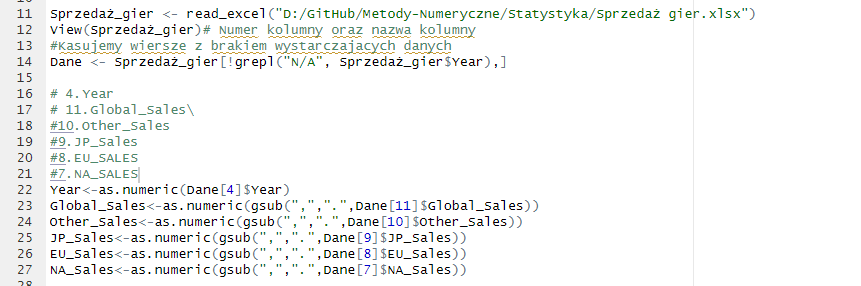
\includegraphics[scale=0.6]{Zad0}
	\newpage
	
	\section{Własności zmiennych (1)}
	Miary tendencji centralnej:\\
	\begin{table}[h]
		\centering
		\begin{tabular}{|c|c|c|c|c|c|c|}
			\hline
			\multicolumn{1}{|l|}{} & Year                             & Global Sale  &JP Sale      &EU Sale & NA sale & Other Sale              \\ \hline
			Średnia               & \cellcolor[HTML]{FFFFFF}2006.406 & \cellcolor[HTML]{FFFFFF}0.5402315 & \cellcolor[HTML]{FFFFFF} 0.07866111  & \cellcolor[HTML]{FFFFFF} 0.1475544 & \cellcolor[HTML]{FFFFFF} 0.07866111& \cellcolor[HTML]{FFFFFF} 0.04832547    \\ \hline
			Mediana                & \cellcolor[HTML]{FFFFFF}2007     & \cellcolor[HTML]{FFFFFF}0.17  & \cellcolor[HTML]{FFFFFF}0& \cellcolor[HTML]{FFFFFF}0.02& \cellcolor[HTML]{FFFFFF}0.08& \cellcolor[HTML]{FFFFFF}0.01   \\ \hline
			Moda                   & \cellcolor[HTML]{FFFFFF}2009     & \cellcolor[HTML]{FFFFFF}0.02    & \cellcolor[HTML]{FFFFFF}0  & \cellcolor[HTML]{FFFFFF}0  & \cellcolor[HTML]{FFFFFF}0  & \cellcolor[HTML]{FFFFFF}0      \\ \hline
		\end{tabular}
	\end{table}
	W powyższej tabelce najbardziej wydaje się wyróżniać średnia dla sprzedaży gier w Europie. Jest ona zauważalnie większa od wszystkich pozostałych regionów. Pomimo tego, mediana Stanów Zjednoczonych jest 4 razy większa niż Europie. Być może, może to być spowodowane tym, że Europejczycy wolą grać w węższą listę tytułów. Nie jest to jednak sprawą naszych późniejszych testów.\\ 
	Miary położenia:\\
	\begin{table}[h]
		\centering
		\begin{tabular}{|ccccc|}
			\hline
			\multicolumn{5}{|c|}{Kwartyl Year}                                                                                                                                                             \\ \hline
			\multicolumn{1}{|c|}{0\%}                          & \multicolumn{1}{c|}{25\%}                         & \multicolumn{1}{c|}{50\%} & \multicolumn{1}{c|}{75\%}                         & 100\% \\ \hline
			\multicolumn{1}{|c|}{\cellcolor[HTML]{FFFFFF}1980} & \multicolumn{1}{c|}{\cellcolor[HTML]{FFFFFF}2003} & \multicolumn{1}{c|}{2007} & \multicolumn{1}{c|}{\cellcolor[HTML]{FFFFFF}2010} & 2020  \\ \hline

			\multicolumn{5}{|c|}{Kwartyl Global Sale}                                                                                                      \\ \hline
			\multicolumn{1}{|c|}{0\%}                          & \multicolumn{1}{c|}{25\%} & \multicolumn{1}{c|}{50\%} & \multicolumn{1}{c|}{75\%} & 100\% \\ \hline
			\multicolumn{1}{|c|}{\cellcolor[HTML]{FFFFFF}0.01} & \multicolumn{1}{c|}{0.06} & \multicolumn{1}{c|}{0.17} & \multicolumn{1}{c|}{0.48} & 82.74 \\ \hline
		\multicolumn{5}{|c|}{Kwartyl Other Sale}                                                                                                      \\ \hline
		\multicolumn{1}{|c|}{0\%}                          & \multicolumn{1}{c|}{25\%} & \multicolumn{1}{c|}{50\%} & \multicolumn{1}{c|}{75\%} & 100\% \\ \hline
		\multicolumn{1}{|c|}{\cellcolor[HTML]{FFFFFF}0} & \multicolumn{1}{c|}{0} & \multicolumn{1}{c|}{0.01} & \multicolumn{1}{c|}{0.04} & 10.57 \\ \hline
		\multicolumn{5}{|c|}{Kwartyl JP Sale}                                                                                                      \\ \hline
		\multicolumn{1}{|c|}{0\%}                          & \multicolumn{1}{c|}{25\%} & \multicolumn{1}{c|}{50\%} & \multicolumn{1}{c|}{75\%} & 100\% \\ \hline
		\multicolumn{1}{|c|}{\cellcolor[HTML]{FFFFFF}0} & \multicolumn{1}{c|}{0} & \multicolumn{1}{c|}{0} & \multicolumn{1}{c|}{0.04} & 10.22 \\ \hline		
		\multicolumn{5}{|c|}{Kwartyl EU Sale}                                                                                                      \\ \hline
		\multicolumn{1}{|c|}{0\%}                          & \multicolumn{1}{c|}{25\%} & \multicolumn{1}{c|}{50\%} & \multicolumn{1}{c|}{75\%} & 100\% \\ \hline
		\multicolumn{1}{|c|}{\cellcolor[HTML]{FFFFFF}0} & \multicolumn{1}{c|}{0} & \multicolumn{1}{c|}{0.02} & \multicolumn{1}{c|}{0.11} & 29.02 \\ \hline
		\multicolumn{5}{|c|}{Kwartyl NA Sale}                                                                                                      \\ \hline
		\multicolumn{1}{|c|}{0\%}                          & \multicolumn{1}{c|}{25\%} & \multicolumn{1}{c|}{50\%} & \multicolumn{1}{c|}{75\%} & 100\% \\ \hline
		\multicolumn{1}{|c|}{\cellcolor[HTML]{FFFFFF}0} & \multicolumn{1}{c|}{0} & \multicolumn{1}{c|}{0.08} & \multicolumn{1}{c|}{0.24} & 41.49 \\ \hline
\end{tabular}
	\end{table}

Kwartyl pierwszy (kolumna 25\%) informuje, że 25\% obserwacji nie jest więsza niż podana pod nią liczba. Analogicznie dla pozostałych kwartyli.\\

\newpage
	Miary Rozproszenia:
	\begin{table}[h]
		\centering
		\begin{tabular}{|c|c|c|}
			\hline
			\multicolumn{1}{|l|}{}             & Year                                & Global Sale                      \\ \hline
			wariancja                          & \cellcolor[HTML]{FFFFFF}33.97702    & \cellcolor[HTML]{FFFFFF}2.451516 \\ \hline
			odchylenie standardowe             & \cellcolor[HTML]{FFFFFF}5.828981    & 1.565732                         \\ \hline
			wspolczynnik zmiennosci            & 0.002905185                         & \cellcolor[HTML]{FFFFFF}2.898261 \\ \hline
			rozstep kwartylowy                 & \cellcolor[HTML]{FFFFFF}7           & 0.42                             \\ \hline
			Kwartylowy współczynnik zmienności & \cellcolor[HTML]{FFFFFF}0.003487793 & \cellcolor[HTML]{FFFFFF}2.470588 \\ \hline
		\end{tabular}
	\end{table}
	\begin{table}[H]
	\centering
	\begin{tabular}{|c|c|c|c|c|}
		\hline
		\multicolumn{1}{|l|}{}             & Other Sale                                & JP Sale    & EU Sale          & NA Sale              \\ \hline
		wariancja                          & \cellcolor[HTML]{FFFFFF}0.03605648    & \cellcolor[HTML]{FFFFFF}0.09706775 & \cellcolor[HTML]{FFFFFF}0.2588425& \cellcolor[HTML]{FFFFFF}0.6750115\\ \hline
		odchylenie standardowe             & \cellcolor[HTML]{FFFFFF}0.1898854  & 0.311557       & \cellcolor[HTML]{FFFFFF}0.5087657    & \cellcolor[HTML]{FFFFFF}0.8215909             \\ \hline
		wspolczynnik zmiennosci            & 3.929303                       & \cellcolor[HTML]{FFFFFF}3.96075 & \cellcolor[HTML]{FFFFFF}3.447988 & \cellcolor[HTML]{FFFFFF}3.095496\\ \hline
		rozstep kwartylowy                 & \cellcolor[HTML]{FFFFFF}0.04           & 0.04   & \cellcolor[HTML]{FFFFFF}0.11     & \cellcolor[HTML]{FFFFFF}0.24                         \\ \hline
		Kwartylowy współczynnik zmienności & \cellcolor[HTML]{FFFFFF}4 & \cellcolor[HTML]{FFFFFF}Inf& \cellcolor[HTML]{FFFFFF} 5.5 & \cellcolor[HTML]{FFFFFF} 3\\ \hline
	\end{tabular}
\end{table}
Wariancja wskazuje na to, że rozproszenie w każdym z regionów jest różne. Po raz kolejny zauważamy, że w Stanach Zjednoczonych rozproszenie tych zmiennych jest najbardziej widoczne.
Odchylenie standardowe, podobnie jak wariancja, wskazuje na umiarkowane rozrzucenie obserwacji wokół średniej.\\
	Kod w R:\newpage
	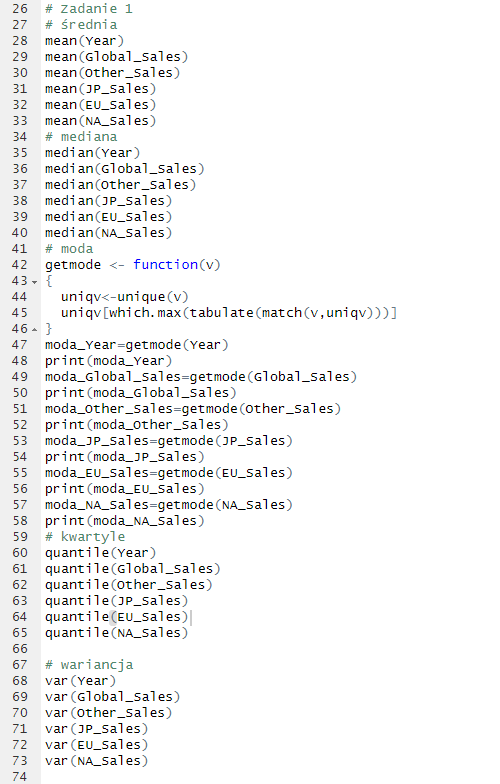
\includegraphics[scale=0.6]{Zad1}\\
	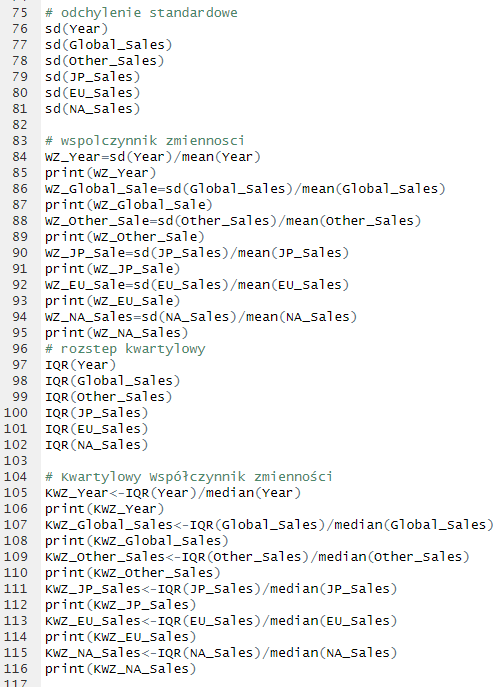
\includegraphics[scale=0.6]{Zad1B}
	
	\newpage
	\section{Miary klasyczne i nieklasyczne (2)}
	\begin{table}[h]
		\centering
		\begin{tabular}{|c|c|c|}
			\hline
			\multicolumn{1}{|l|}{}                              & Year                             & Global Sales                     \\ \hline
			\multicolumn{3}{|c|}{Miary klasyczne}                                                                                                           \\ \hline
			\multicolumn{1}{|c|}{Moment trzeci centralny (\(\mu_{3}\))}       & \multicolumn{1}{c|}{\cellcolor[HTML]{FFFFFF}-198.522}  & \cellcolor[HTML]{FFFFFF}66.47233 \\ \hline
			\multicolumn{1}{|c|}{Moment trzeci względny (\(\alpha_{3}\))}        & \multicolumn{1}{c|}{\cellcolor[HTML]{FFFFFF}-1.002376} & \cellcolor[HTML]{FFFFFF}17.31764 \\ \hline
			\multicolumn{1}{|c|}{Moment czwarty centralny (\(\mu_{4}\))}      & \multicolumn{1}{c|}{\cellcolor[HTML]{FFFFFF}5595.161}  & \cellcolor[HTML]{FFFFFF}3605.495 \\ \hline
			\multicolumn{1}{|c|}{Moment czwarty względny (\(\alpha_{4}\))}       & \multicolumn{1}{c|}{\cellcolor[HTML]{FFFFFF}4.846653}  & \cellcolor[HTML]{FFFFFF}599.9227 \\ \hline
			\multicolumn{3}{|c|}{Miary nieklasyczne}                                                                                                        \\ \hline
			\multicolumn{1}{|c|}{Kwartyl wpolczynnik skosnosci} & \multicolumn{1}{c|}{\cellcolor[HTML]{FFFFFF}-1.002376} & \cellcolor[HTML]{FFFFFF}17.31764 \\ \hline
		\end{tabular}
	\end{table}
\begin{table}[h]
	\centering
	\begin{tabular}{|c|c|c|c|c|}
		\hline
		\multicolumn{1}{|l|}{}                              & Other  Sales                           & JP Sales      & EU Sales     & NA Sales         \\ \hline
		\multicolumn{5}{|c|}{Miary klasyczne}                                                                                                           \\ \hline
		\multicolumn{1}{|c|}{Moment trzeci centralny (\(\mu_{3}\))}       & \multicolumn{1}{c|}{\cellcolor[HTML]{FFFFFF}0.1651514}  & \cellcolor[HTML]{FFFFFF}0.3367088& \cellcolor[HTML]{FFFFFF}2.474508& \cellcolor[HTML]{FFFFFF}10.40093 \\ \hline
		\multicolumn{1}{|c|}{Moment trzeci względny (\(\alpha_{3}\))}        & \multicolumn{1}{c|}{\cellcolor[HTML]{FFFFFF}24.12168} & \cellcolor[HTML]{FFFFFF}11.13376& \cellcolor[HTML]{FFFFFF}18.79037& \cellcolor[HTML]{FFFFFF}18.75449 \\ \hline
		\multicolumn{1}{|c|}{Moment czwarty centralny (\(\mu_{4}\))}      & \multicolumn{1}{c|}{\cellcolor[HTML]{FFFFFF}1.321612}  & \cellcolor[HTML]{FFFFFF}1.832858& \cellcolor[HTML]{FFFFFF}50.2929& \cellcolor[HTML]{FFFFFF}294.7414 \\ \hline
		\multicolumn{1}{|c|}{Moment czwarty względny (\(\alpha_{4}\))}       & \multicolumn{1}{c|}{\cellcolor[HTML]{FFFFFF}1016.57}  & \cellcolor[HTML]{FFFFFF}27.35631 & \cellcolor[HTML]{FFFFFF}194.5265& \cellcolor[HTML]{FFFFFF}646.8726\\ \hline
		\multicolumn{5}{|c|}{Miary nieklasyczne}                                                                                                        \\ \hline
		\multicolumn{1}{|c|}{Kwartyl wpolczynnik skośności} & \multicolumn{1}{c|}{\cellcolor[HTML]{FFFFFF}24.12168} & \cellcolor[HTML]{FFFFFF}11.13376 & \cellcolor[HTML]{FFFFFF}18.79037 & \cellcolor[HTML]{FFFFFF}18.75449 \\ \hline
	\end{tabular}
\end{table}
Zmienna Year:\\
Moment trzeci centralny jest mniejszy od 0, moment trzeci względny jest w przedziale -2 i 2, a moment czwarty względny jest większy niż 3. Czyli dla momentu 3 jest zatem mała skośność. Dla momentu 4 jest to rozkład wysmukły. Jest prawoskośny (współczynnik skośności ujemny oraz moment trzeci centralny). \\
       Zmienne Global Sales, Other Sales, JP Sales, EU Sales, Na Sales wyglądają podobnie:\\
Moment trzeci centralny jest większy od 0, moment trzeci względny jest wysoki, wyższy od 2, a moment czwarty względny jest bardzo duży. Występuje duża skośność, oraz rozkład smukły. Są prawoskośne, ponieważ momenty trzecie centralne oraz współczynniki skośności są dodatnie.\\
\newpage
	Kod w R:\\
	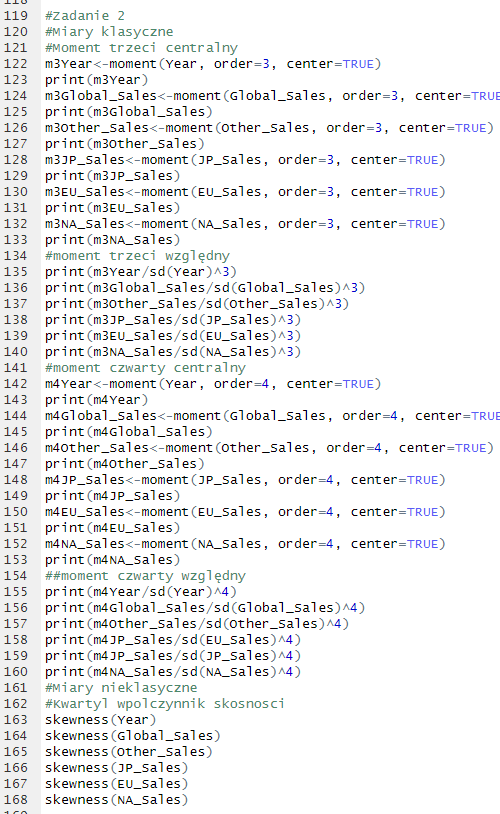
\includegraphics[scale=0.7]{Zad2}
	
	\newpage
	\section{Histogramy (3)}
	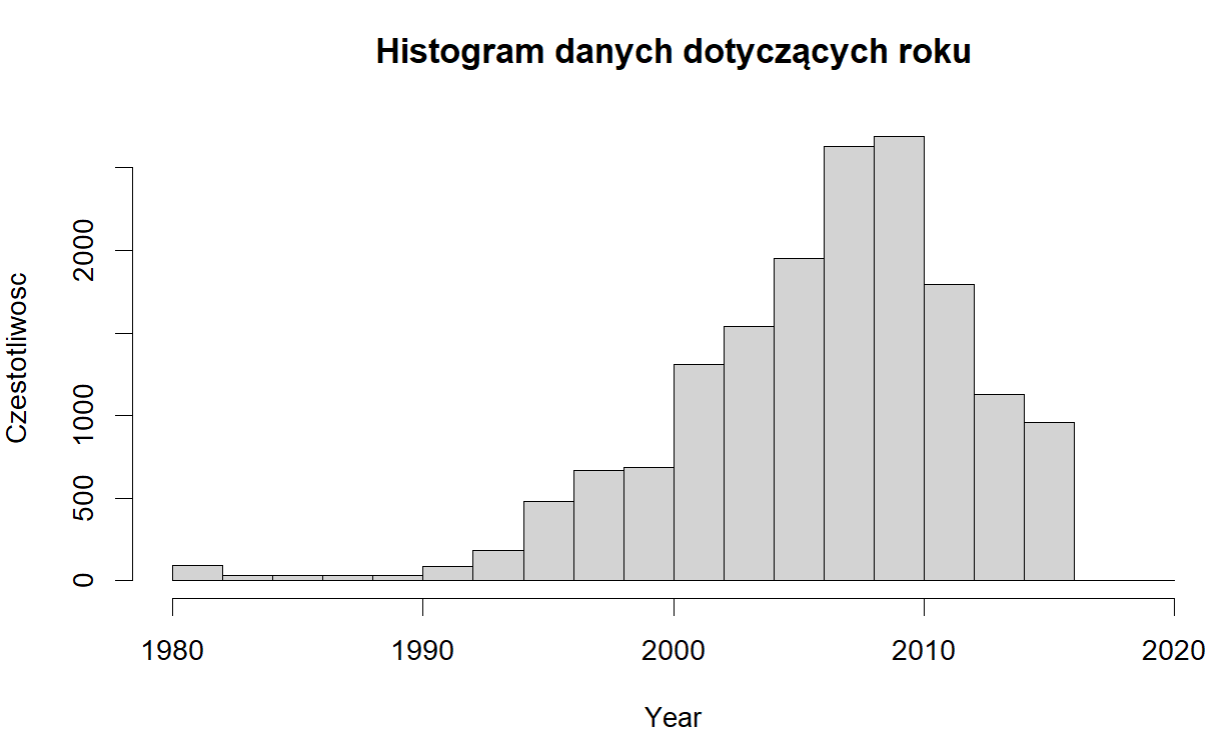
\includegraphics[scale=0.25]{HistogramRok}\\
	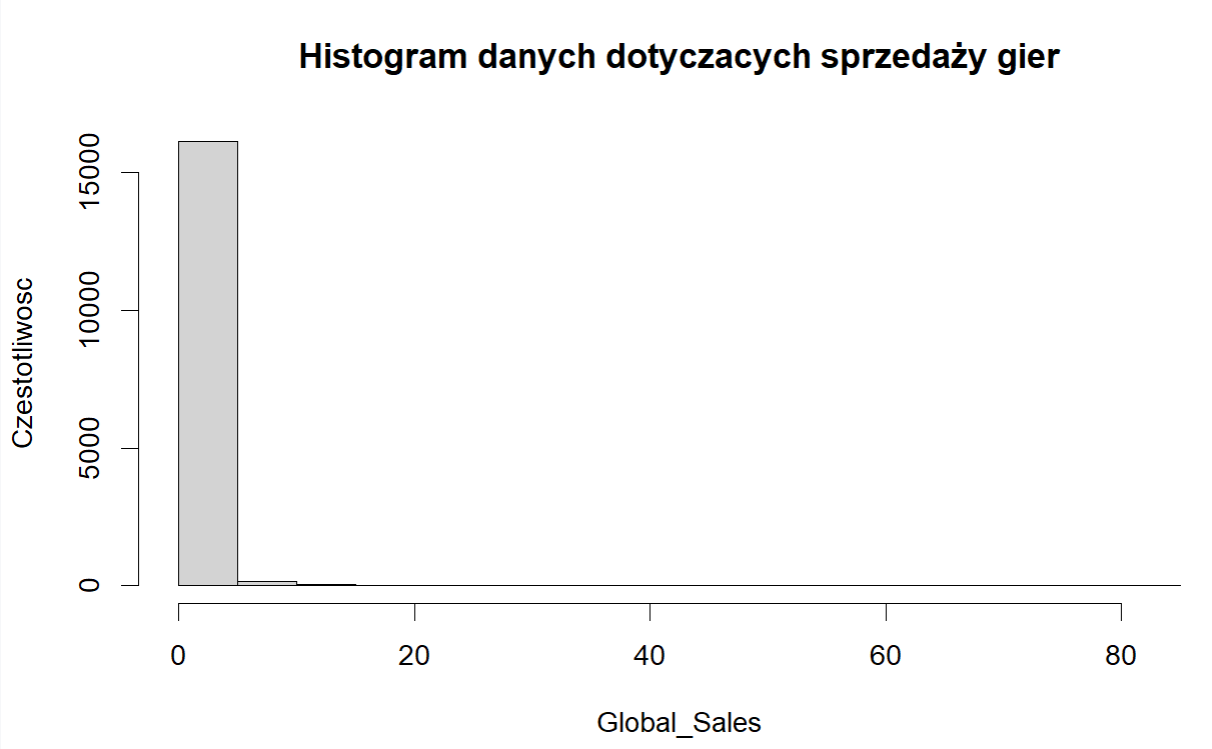
\includegraphics[scale=0.4]{HistogramSales}\\
	\includegraphics[scale=0.6]{HistogramOther}\\
	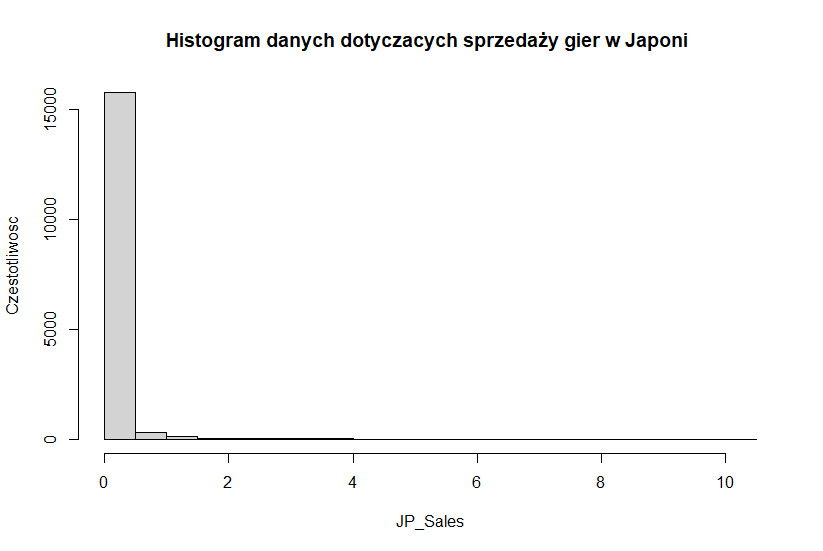
\includegraphics[scale=0.6]{HistogramJP}\\
	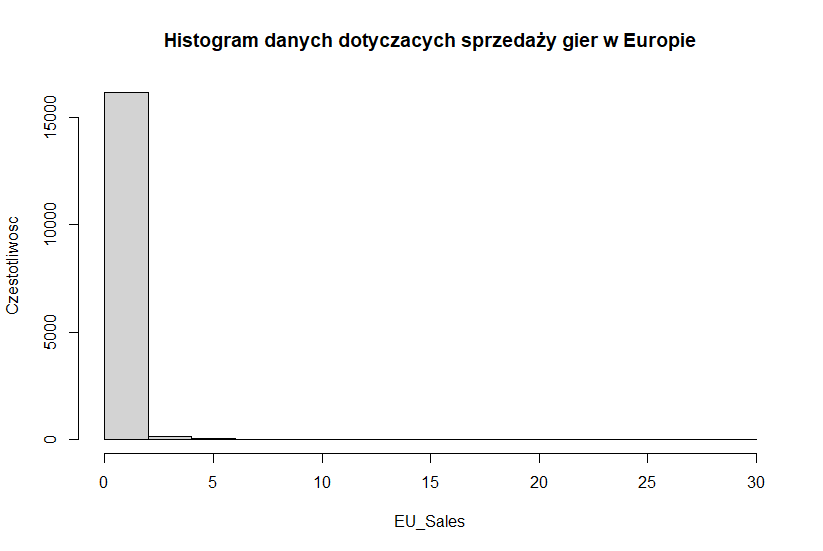
\includegraphics[scale=0.6]{HistogramEU}\\
	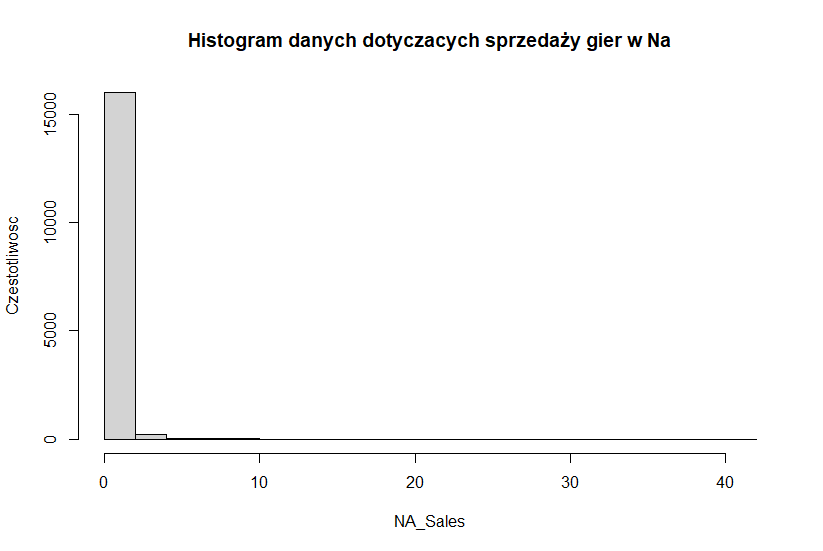
\includegraphics[scale=0.6]{HistogramNA}\\
	Kod w R:\\
	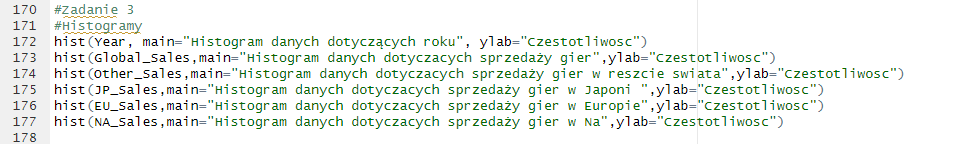
\includegraphics[scale=0.5]{Zad3}
	\newpage
	
	\section{Testy zgodności z rozkładem normalnym (4)}
	
	\(H_0\)-hipoteza zerowa, dane pochodzą z rozkładu normalnego.\\
	\(H_A\)-hipoteza alternatywna, dane nie pochodzą z rozkładu normalnego.\\
Zakładamy poziom istotności a=0,05.\\
		Nie udało się przeprowadzić testu "Shapiro test" oraz "Cramer-von Mises" ze względu na dane (R nie zwrócił nam ich wartości). Problemy być może mogła sprawiać zbyt duża liczba wierszy w bazie danych. (W kodzie R, skopiowałem treść napotkanych błędów).\\
	Wartość teoretyczna testu Kolmogorov-Smirnov wynosi u nas około 0.0105556...\\ 
	Wartość teoretyczna testu Anderson-Darling wynosi u nas około 1.225...\\ 
	\begin{table}[H]
		\centering
		\begin{tabular}{|c|c|}
			\hline
			\rowcolor[HTML]{00FFFF} 
			Data:              & Year                            \\ \hline
			p-value (dla każdego)            & \textless{}2.2e-16              \\ \hline
			Kolmogorov-Smirnov & \cellcolor[HTML]{FFFFFF}0.1044  \\ \hline
			\rowcolor[HTML]{FFFFFF} 
			Anderson-Darling   & 170.87                          \\ \hline
			\rowcolor[HTML]{00FFFF} 
			Data:              & Global Sales                    \\ \hline
			p-value (dla każdego)            & \textless{}2.2e-16              \\ \hline
			Kolmogorov-Smirnov & \cellcolor[HTML]{FFFFFF}0.36744 \\ \hline
			Anderson-Darling   & \cellcolor[HTML]{FFFFFF}3232.7  \\ \hline
			\rowcolor[HTML]{00FFFF} 
			Data:              & Other Sales                    \\ \hline
			p-value (dla każdego)            & \textless{}2.2e-16              \\ \hline
			Kolmogorov-Smirnov & \cellcolor[HTML]{FFFFFF} 0.39956 \\ \hline
			Anderson-Darling   & \cellcolor[HTML]{FFFFFF}3763.6  \\ \hline
			\rowcolor[HTML]{00FFFF} 
			Data:              & JP Sales                    \\ \hline
			p-value (dla każdego)            & \textless{}2.2e-16              \\ \hline
			Kolmogorov-Smirnov & \cellcolor[HTML]{FFFFFF} 0.40034 \\ \hline
			Anderson-Darling   & \cellcolor[HTML]{FFFFFF}4003  \\ \hline
			\rowcolor[HTML]{00FFFF} 
						Data:              & EU Sales                    \\ \hline
			p-value (dla każdego)            & \textless{}2.2e-16              \\ \hline
			Kolmogorov-Smirnov & \cellcolor[HTML]{FFFFFF} 0.3859 \\ \hline
			Anderson-Darling   & \cellcolor[HTML]{FFFFFF}3515  \\ \hline
			\rowcolor[HTML]{00FFFF} 
			Data:              & NA Sales                    \\ \hline
			p-value (dla każdego)            & \textless{}2.2e-16              \\ \hline
			Kolmogorov-Smirnov & \cellcolor[HTML]{FFFFFF}  0.37333 \\ \hline
			Anderson-Darling   & \cellcolor[HTML]{FFFFFF}3206  \\ \hline
		\end{tabular}
	\end{table}
	W każdym z testów uzyskaliśmy p-value mniejsze od 2.2e-16, zatem \(p<a=0.05\) (czyli maksymalnego dopuszczenia błędu 1 rodzaju).
	Mamy zatem podstawy, żeby odrzucić hipotezę zerową. Rozkład danych nie jest normalny.
	
	Kod w R:\\
	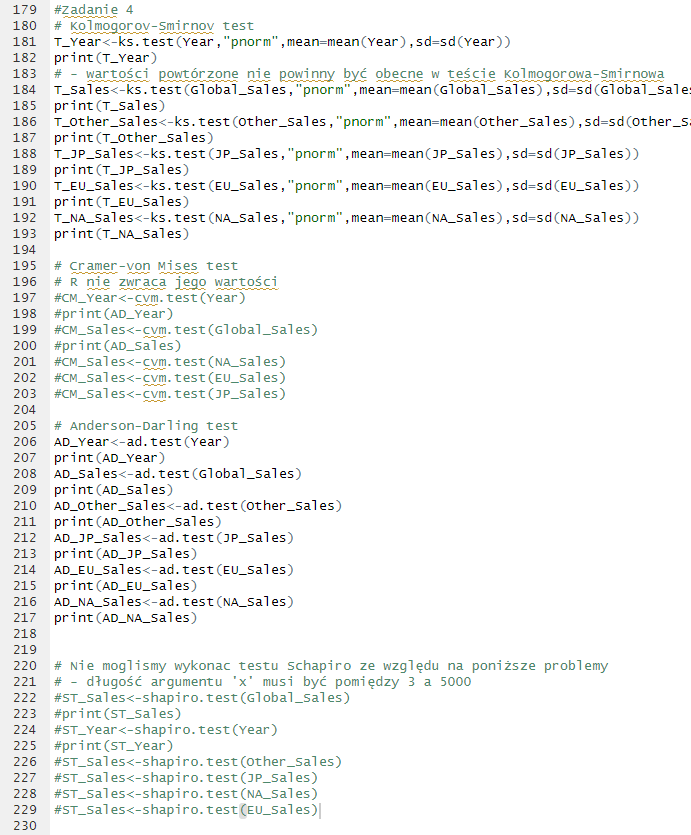
\includegraphics[scale=0.5]{Zad4}
	\newpage
	
	\section{Test Mardia (6)}
	\(H_0\)-hipoteza zerowa, wektor losowy złożony z danych ma rozkład normalny.\\
	\(H_A\)-hipoteza alternatywna, wektor losowy nie ma rozkładu normalnego.\\
Przyjmujemy taki sam poziom istotności jak w poprzednich testach.\\
	\begin{table}[H]
		\centering
		\begin{tabular}{|cccc|}
			\hline
			\multicolumn{4}{|c|}{Mardia test}                                                                                                                                                                        \\ \hline
			\multicolumn{1}{|l|}{}                                 & \multicolumn{1}{c|}{\cellcolor[HTML]{FFFFFF}Beta-hat} & \multicolumn{1}{c|}{\cellcolor[HTML]{FFFFFF}kappa}      & \cellcolor[HTML]{FFFFFF}p-val \\ \hline

\multicolumn{4}{|c|}{Year, Global Sales}                                                                                                                                                                       \\ \hline

			\multicolumn{1}{|c|}{\cellcolor[HTML]{FFFFFF}Skewness} & \multicolumn{1}{c|}{\cellcolor[HTML]{FFFFFF}303.2542} & \multicolumn{1}{c|}{\cellcolor[HTML]{FFFFFF}825205.149} & 0                             \\ \hline

			\multicolumn{1}{|c|}{\cellcolor[HTML]{FFFFFF}Kurtosis} & \multicolumn{1}{c|}{\cellcolor[HTML]{FFFFFF}612.9963} & \multicolumn{1}{c|}{\cellcolor[HTML]{FFFFFF}9663.089}   & 0                             \\ \hline


\multicolumn{4}{|c|}{Year, Other Sales}                                                                                                                                                                       \\ \hline

			\multicolumn{1}{|c|}{\cellcolor[HTML]{FFFFFF}Skewness} & \multicolumn{1}{c|}{\cellcolor[HTML]{FFFFFF}585.515} & \multicolumn{1}{c|}{\cellcolor[HTML]{FFFFFF}1593283.93} & 0                             \\ \hline

			\multicolumn{1}{|c|}{\cellcolor[HTML]{FFFFFF}Kurtosis} & \multicolumn{1}{c|}{\cellcolor[HTML]{FFFFFF}1026.503} & \multicolumn{1}{c|}{\cellcolor[HTML]{FFFFFF}16267.67}   & 0                             \\ \hline

\multicolumn{4}{|c|}{Year, JP Sales}                                                                                                                                                                       \\ \hline

			\multicolumn{1}{|c|}{\cellcolor[HTML]{FFFFFF}Skewness} & \multicolumn{1}{c|}{\cellcolor[HTML]{FFFFFF}128.1869} & \multicolumn{1}{c|}{\cellcolor[HTML]{FFFFFF}348817.940} & 0                             \\ \hline

			\multicolumn{1}{|c|}{\cellcolor[HTML]{FFFFFF}Kurtosis} & \multicolumn{1}{c|}{\cellcolor[HTML]{FFFFFF}208.8988} & \multicolumn{1}{c|}{\cellcolor[HTML]{FFFFFF}3208.785}   & 0                             \\ \hline

\multicolumn{4}{|c|}{Year, EU Sales}                                                                                                                                                                       \\ \hline

			\multicolumn{1}{|c|}{\cellcolor[HTML]{FFFFFF}Skewness} & \multicolumn{1}{c|}{\cellcolor[HTML]{FFFFFF}354.0930} & \multicolumn{1}{c|}{\cellcolor[HTML]{FFFFFF}963546.20} & 0                             \\ \hline

			\multicolumn{1}{|c|}{\cellcolor[HTML]{FFFFFF}Kurtosis} & \multicolumn{1}{c|}{\cellcolor[HTML]{FFFFFF}757.0341} & \multicolumn{1}{c|}{\cellcolor[HTML]{FFFFFF}11963.68}   & 0                             \\ \hline

\multicolumn{4}{|c|}{Year, NA Sales}                                                                                                                                                                       \\ \hline

			\multicolumn{1}{|c|}{\cellcolor[HTML]{FFFFFF}Skewness} & \multicolumn{1}{c|}{\cellcolor[HTML]{FFFFFF}354.9592} & \multicolumn{1}{c|}{\cellcolor[HTML]{FFFFFF}965903.1} & 0                             \\ \hline

			\multicolumn{1}{|c|}{\cellcolor[HTML]{FFFFFF}Kurtosis} & \multicolumn{1}{c|}{\cellcolor[HTML]{FFFFFF}660.8681} & \multicolumn{1}{c|}{\cellcolor[HTML]{FFFFFF}10427.7}   & 0                             \\ \hline

		\end{tabular}
	\end{table}
	Otrzymano \(p=0<a=0,05\), zatem wektor losowy nie ma rozkładu normalnego. Hipoteza zerowa została odrzucona, zatem obliczamy współczynnik korelacji rang.
	
	Kod w R:\\
	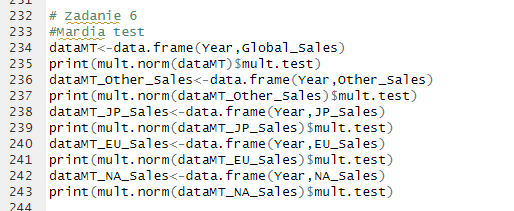
\includegraphics[scale=0.6]{Zad6}
	\newpage
	\section{Współczynnik korelacji rang Spearmana (8)}
	\(H_0\)-hipoteza zerowa, \(r_{s}=0\).\\
	\(H_A\)-hipoteza alternatywna, \(r_{s}\neq0\).\\
Im bliżej współczynnik zbliża się do 1, tym bardziej powiązane są zmienne.
Wartość teoretyczna testu Spearmana wyniosła u nas około 0.07... (miałem problem, by otrzymać dokładną liczbę dla tak wielu próbek)\\ 

	Dla sprzedarzy w Japoni:\\
	Wynik testu Spearmana:\\
	\(S=7.1842e+11\)\\
	\(p-value =0.2197\)\\
	Otrzymano wspłczynnik korelacji rang Spearmana \(rho= 0.0096053322 \in (-1;1)\).\\
{\color{red}\textbf{Oznacza to, że dla zmiennych Year oraz JP\_Sales nie odrzucamy hipotezy zerowej! (ponieważ \(p-value>alpha\))} }
\\
\\
	Dla pozostałych zmiennych nie udało się nam uzyskać \(p-value > a=0,05\).\\
	Dla zmiennej Global Sale:\\
	Wynik testu Spearmana:\\
	\(S=8.351e+11\)\\
	\(p-value < 2.2e-16\)\\
	Otrzymano wspłczynnik korelacji rang Spearmana \(rho=-0.1512482 \in (-1;1)\).\\
	Dla sprzedarzy w NA:\\
	Wynik testu Spearmana:\\
	\(S= 8.2192e+11\)\\
	\(p-value < 2.2e-16\)\\
	Otrzymano wspłczynnik korelacji rang Spearmana \(rho= -0.133088  \in (-1;1)\).\\
	Dla sprzedarzy w Europy:\\
	Wynik testu Spearmana:\\
	\(S=7.6726e+11\)\\
	\(p-value = 1.558e-13\)\\
	\(rho: -0.05772944   \)\\
	Otrzymano wspłczynnik korelacji rang Spearmana \(rho= -0.05772944   \in (-1;1)\).\\
	Dla sprzedarzy na reszce świata:\\
	Wynik testu Spearmana:\\
	\(S=6.8496e+111\)\\
	\(p-value =  1.037e-12\)\\	
	\(rho: 0.05572604   \)\\
	Otrzymano wspłczynnik korelacji rang Spearmana \(rho= 0.05572604   \in (-1;1)\).\\

Dla tych zmiennych Hipoteza alternatywna: rho nie jest równe 0.\\
	Test korelacji dla nich wyliczył wartość p, będącą mniejszą od założonej wartości a. Oznacza to, żę odrzucamy hipotezę zerową na rzecz hipotezy alternatywnej.

	Kod w R:\\
	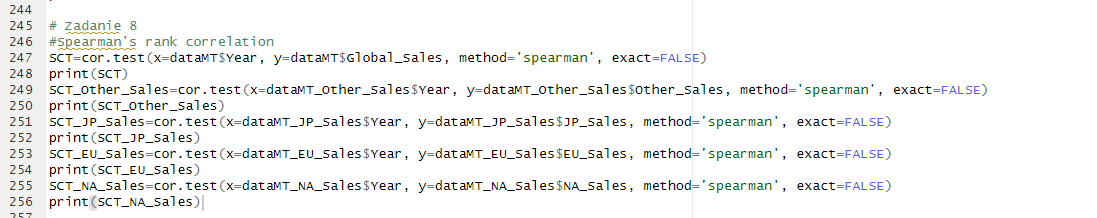
\includegraphics[scale=0.5]{Zad8}
	
	\section{Test Chi-kwadrat oraz współczynnik kontyngencji V Cramera (11)}
Zakładamy poziom istotności a=0,05.
Wartość teoretyczna testu Chi-kwadrat wyniosła u nas około 16482... \\ 
	\(H_0\)-hipoteza zerowa, dwie zmienne klasyfikujące są wzajemnie zależne.\\
	\(H_A\)-hipoteza alternatywna, dwie zmienne klasyfikujące nie są wzajemnie zależne.\\
	Wynik testu Chi-Squared (Reszta świata):\\
	\(X-squared = 5758.6\)\\
	\(df=5928\)\\
	\(p-value =0.9412\)\\
{\color{red}\textbf{Oznacza to, że dla zmiennych Year oraz Other\_Sales nie odrzucamy hipotezy zerowej! (ponieważ \(p-value>alpha\))} }
Jest to prawdopodobne, ponieważ regiony mniej rozwinięte, mogą mieć mniejsze możliwości na zakup najnowszych gier.\\
Dla pozostałych zmiennych:\\
Test chi-kwadrat wyliczył wartość \(p<2.2e-16\). Odrzucamy hipotezę zerową na rzecz hipotezy alternatywnej. \\
	Wynik testu Chi-Squared (Cały Świat):\\
	\(X-squared = 49801\)\\
	\(df=23560\)\\
	\(p-value < 2.2e-16\)\\
	Wynik testu Chi-Squared (Japonia):\\
	\(X-squared = 47852\)\\
	\(df=9234\)\\
	\(p-value < 2.2e-16\)\\
	Wynik testu Chi-Squared (Europa):\\
	\(X-squared = 15680\)\\
	\(df=11552\)\\
	\(p-value < 2.2e-16\)\\
	Wynik testu Chi-Squared (NA):\\
	\(df=15466\)\\
	\(p-value < 2.2e-16\)\\
	%\section{Zadanie 11 b}
	Współczynnik kontyngencji V Cramera wyniósł u nas 
	\(X-squared = 36672\)\\0.283317 dla całego świata, natomiast dla poszególnych regionów:
	\begin{itemize}
		\item Japonia: $0.2777191$
		\item Europa: $0.1589726$
		\item NA: $0.2431211$
		\item Reszta świata: $0.09634113$
	\end{itemize}
Współczynnik V Cramera daje w wyniku wartości pomiędzy 0 a 1. Im wynik jest bliżej 0, tym słabszy jest związek między badanymi cechami, a im bliżej jest 1, tym silniejszy jest związek między badanymi cechami.\\
	Stwierdza się wiec, że powiązanie między zmiennymi jest na niskim poziomie, ale nie zerowe.\\
Nie należy jednak na tej podstawie wyciągać zbyt daleko idących wniosków.\\
	Kod w R:\\
	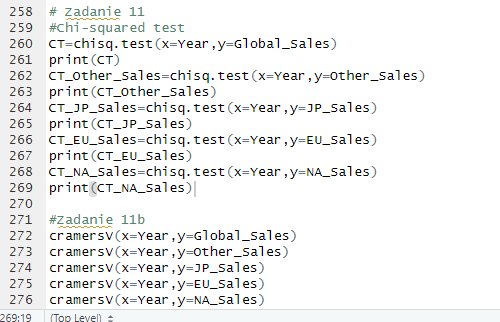
\includegraphics[scale=0.7]{Zad11}
	
\end{document}